\chapter{Feature selection}

In order to create an effective predictive model one must first select a set of features used to produce each classification. Both a science and an art, this process involves intuition, theory and a hefty amount of trial-and-error. Although a seemingly daunting task, for a model to be effective the feature selection procedure is key, and a carefully considered selection often generates significantly better results than one hastily put together. 

Ideally, one seeks a small set of variables which accurately captures the information content in a larger set of data. After reducing the number of features into a more manageable format it is then possible to obtain good results with significantly less computational load than if no feature selection had been considered. Furthermore, the feature selection process allows us to pinpoint what data characteristics we wish to monitor, and subsequently which data characteristics we can disregard. 

\section{Desirable traits}

In the present case the objective is to capture defining characteristics of a surface using one dimensional data obtained from a radar sensor placed some small distance above the surface of interest. Furthermore, the sensor is moving along some direction parallell to the surface plane, thus continuously altering the sensors surroundings. One may split up the possible methods of characterizing this data obtained through this process into two main categories: Methods which aim at capturing the overall spatial signal form, and methods which examine the temporal changes in radar response. 

The first of the two is straight forward; if the scattering surface can be assumed to maintain some defining characteristics at any given point time one could simply extract features relating to these characteristics to generate a classification. Say for example we are presented two surfaces with equivalent reflective properties but where one is rough and the other is smooth. For the smooth surface the scatterers behave more predictably than the rugged surface. This would mean that the main portion of scattered electromagnetic waves will scatter at the

one would expect to receive a strong response from a electromagnetic pulse sent at a zero degree angle of incidence. If one instead sends a pulse at a higher angle of incidence, one would expect the opposite as the scatterers of the smooth surface would primarily scatter away from the sensor yielding a weak response. For the rough surface on the other hand, scatterers direct an incoming reflection in a wider array of angles. 

% Fortsätt här


due to the various properties of the scattering surface in the vicinity 

we begin this section with a discussion 



In order to make sense of data one must impose some reasonable assumptions. 
\\ 
One idea is to view each measurement, taken at time instance $t$ at range $r$ for material $m$, as drawn from some 
complex distribution specific for that combination of $r$ and $s$ but independent of time of sampling $t$. 
\\
Yada yada there is two combatting ideas here

\section{Preprocessing}

\subsection{Using multiple sweeps for feature selection}

In the radar system multiple sources of noise are introduced.
\\ \\
Noise sources: Thermal emissions of target, random currents in electrical components, data quantization, etc. etc. \citep{w_doerry_2016}
\\ \\
In the beginning section of this chapter we introduced two conflicting interpretations of the radar signal. In the first the incomming wavelet is drawn from a complex distribution, and each sweep is independent from the rest. In the second we instead considered that there may be some significant correlations in time to take into account; surface shapes and objects passing by the sensor are detected multiple times in a perhaps predictable and useful manner.  

The first suggest that signal averaging over a number of sweeps should yield a more and more accurate estimate. Thus the first approach greatly benefit from using multiple sweeps to find an average over some predefined number of sweeps.  In order to utilize the time correlations assumed in the second interpretation processing in time is of course demanded, and a number of sweeps need to be analyzed at once to extract features related to this way of viewing the radar response. 

Thus a predefined number is chosen as the number of sweeps used to extract each feature. While each feature may be extracted with higher accuracy, it is done at the price of a lower number of classifications per second. The relation between classification rate $F_c$, sampling speed $F_s$ and sweeps per feature $T_s$ is



\begin{equation}
	F_c = \frac{F_s}{T_s}
\end{equation}

\section{Features}

Fast time and slow time features 



\subsection{Expected signal}
The simplest way of selecting features would be to use plain sweep data as features. While this method requires very little data preprocessing, it does not give very good results (Any comment on how well it performs?). With just a little more effort, a significant improvement can be made by averaging a few sweeps in slow time, as in figure \ref{fig:sweep_average}. This makes the samples more similar.  For range bin $i$, $T$ consecutive samples in slow time are collapsed into one according to

\begin{equation}
	s_i(t_m) = \E\{X_{i,t_m}\} = \frac{1}{T}\sum_{t=0}^{T-1}x(i, t_m + t).
\end{equation}

\begin{figure}[h]
	\centering
	\includegraphics[scale=0.7]{figs_temp/features/sweep_average}
	\caption{}
	\label{fig:sweep_average}
\end{figure}

\subsection{Average energy}
The average energy in a sweep tells us how much energy is reflected back to the radar. Hence it can be regarded as a measure of how good of a reflector the underlying surface is. The energy depends on the shape of the surface, as well as its dielectric constant. Compared to other materials, grass has a very different surface shape, which potentially gives it a very different reflexivity. However, its dielectric constant could also vary a lot depending on whether it is wet or dry, making it hard to guess its reflective properties.

By computing the average energy of single sweeps from different surfaces we see in figure \ref{fig:sweep_energy} that grass reflects much less energy. This indicates that the average sweep energy is a good feature for binary grass/not grass classification. However, in order to get a more robust measure of the average energy we do not only compute the average over selected range bins of a single sweep, but we average over a few consecutive sweeps as well. Mathematically, the feature we end up using becomes
\begin{equation}
	P(t_m) = \frac{1}{NT}\sum_{t=0}^{T-1}\sum_{n=0}^{K-1}x(n, t_m + t)x^*(n, t_m + t),
\end{equation}
where (describe variables)

\begin{figure}[h]
	\centering
	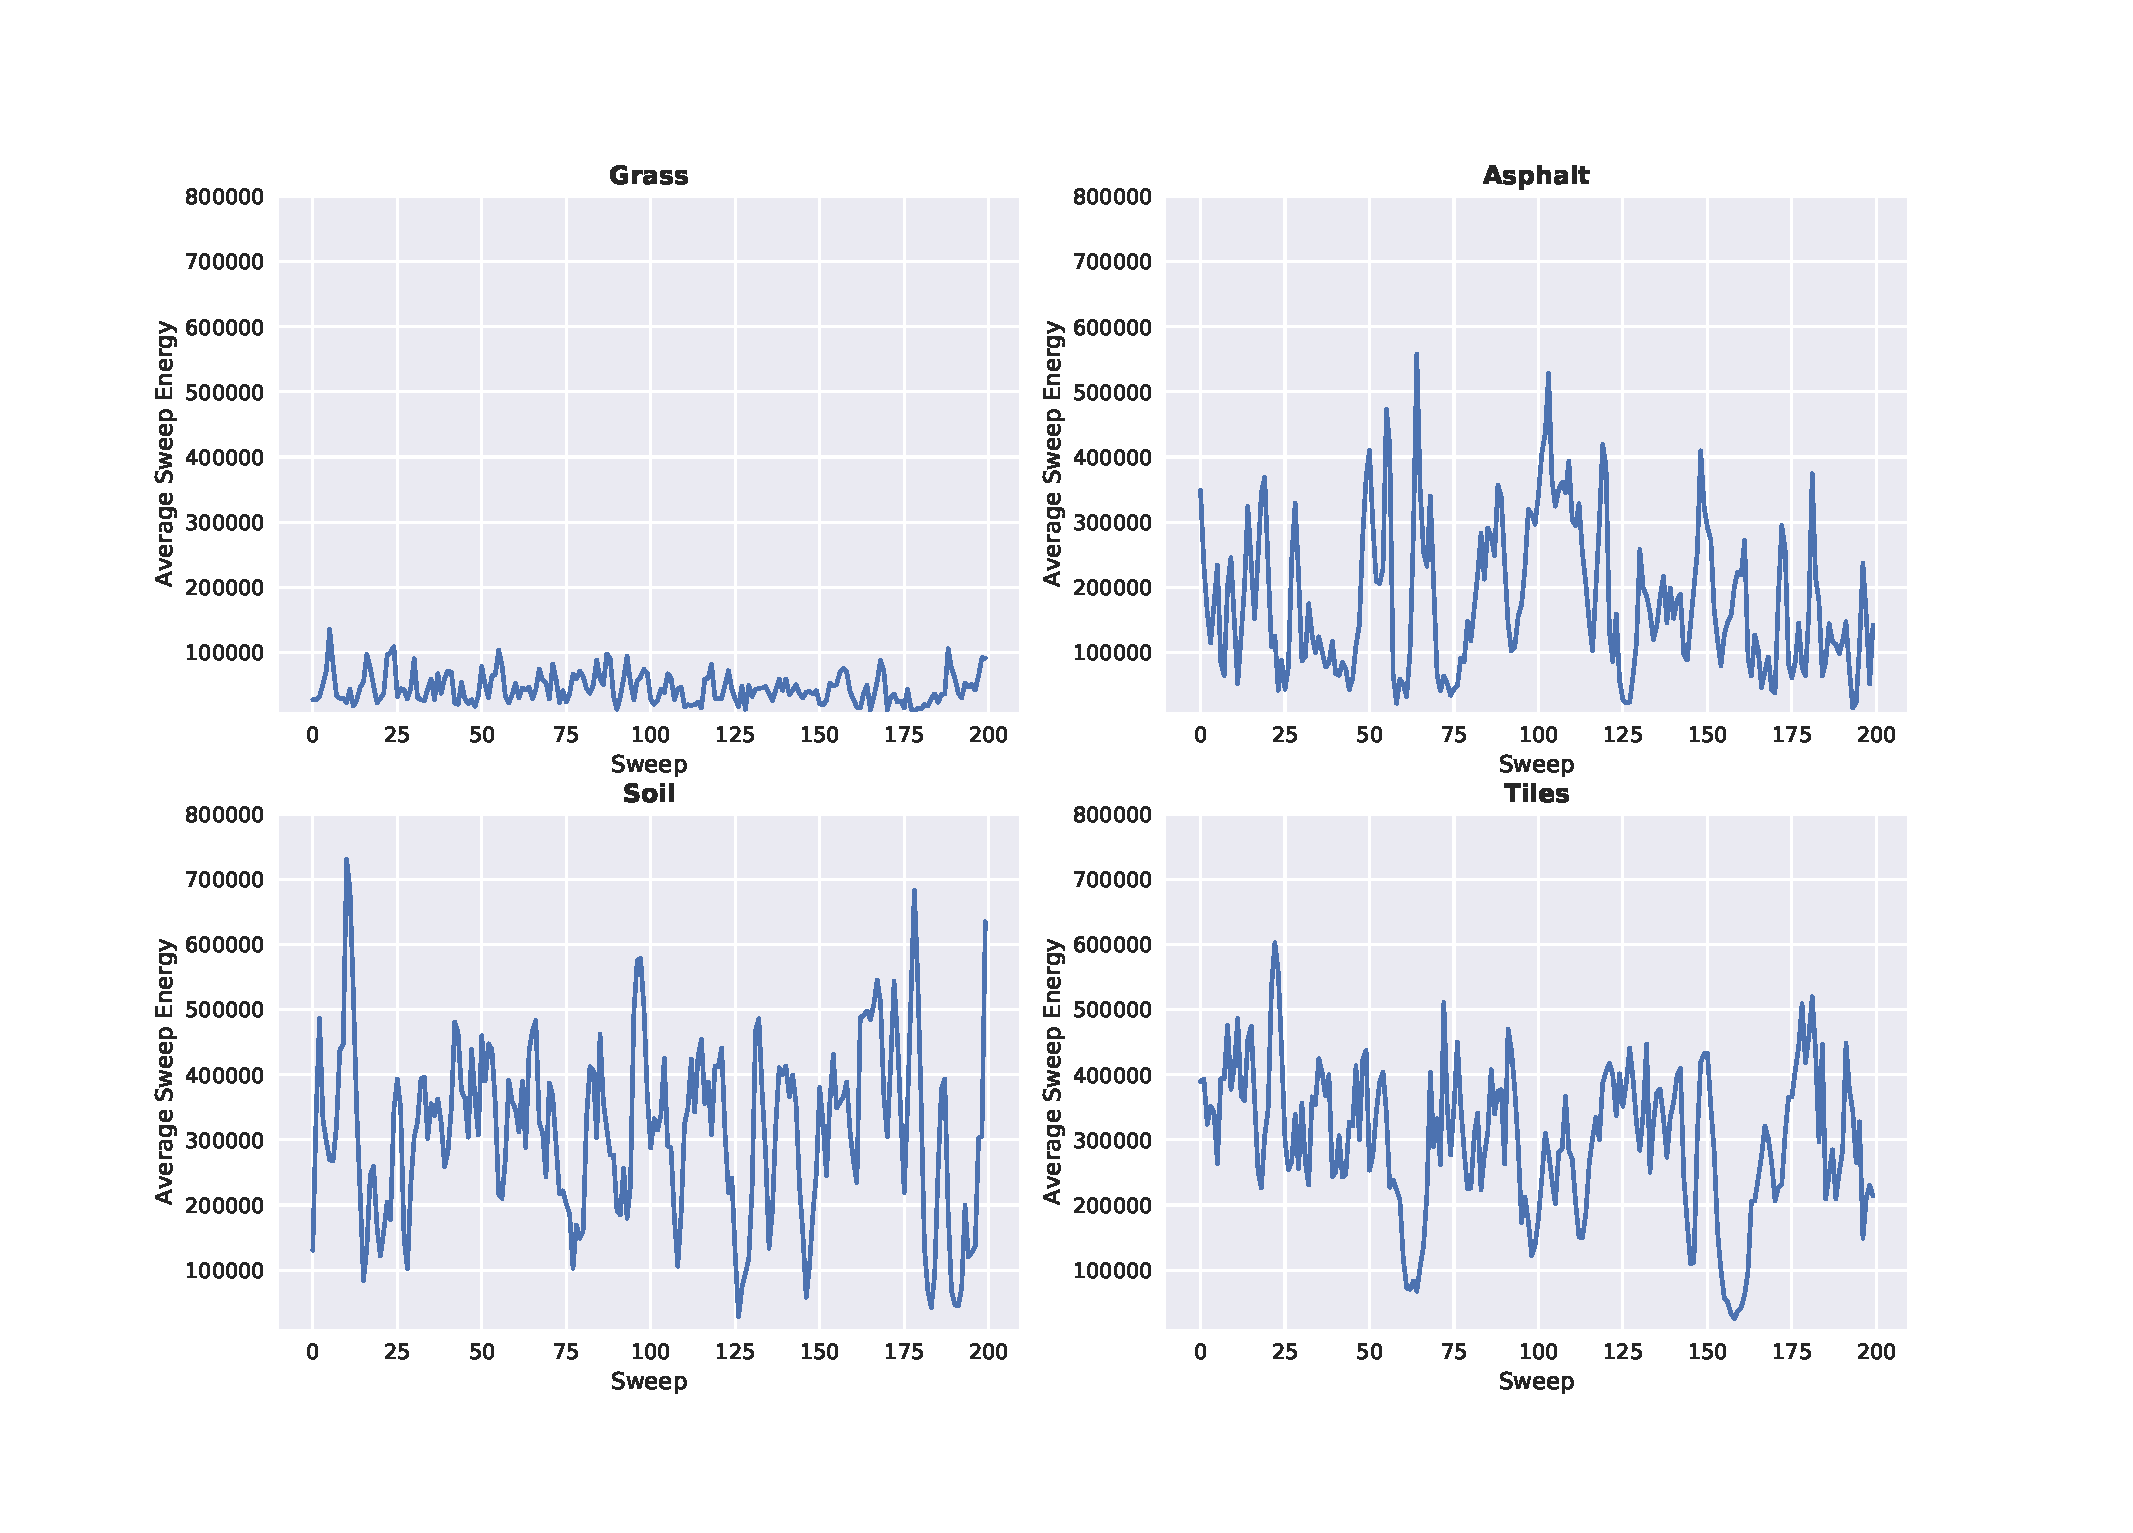
\includegraphics[scale=0.45]{figs_temp/features/sweep_energy}
	\caption{The figure shows the average sweep energy for 200 sweeps and four different materials. All measurements were made during a short period of time. The reflections from the grass surface carry noticeably less energy than those from the other surfaces. }
	\label{fig:sweep_energy}
\end{figure}



\subsection{Fourier Transform}


A "feature box" consisting of $T$ sweeps is selected. Viewing this as a matrix with elements $X_{n,t}$, where $n$ denotes slow time, and $t$ fast time we can write a Fourier transform in slow time at range $r$, within this box as
\begin{equation}
	\mathbb{X}_k^{(r)} = \sum_{n=0}^{T-1}X_{n,r}\exp\Big[-2\pi i\frac{nk}{T}\Big] \quad k=0, ..., T-1
\end{equation}
To avoid aliasing we refer to chapter earlier in report where this is discussed. Mention that $\mathbb{X}_k^{(r)}$, for all $r$, $k$, is flattened to a vector, resulting in one new sample.

\begin{figure}[h]
	\centering
	\includegraphics[scale=0.4]{figs_temp/features/fft}
	\caption{Each plot shows 5 concatenated DFTs, which have all been estimated from 128 consecutive sweeps. This has been done for ranges 7-23 cm, and the materials included in the figure are grass, asphalt, soil and tiles, respectively.}
	\label{fig:fft}
\end{figure}




\subsection{Variance}

Include a discussion about the biased/unbiased estimate \\

Assume $x(n,t)$ are samples from a complex normal distribution $X_{n,t}$. Variance $v_i(t_m)$ at range $i$ at time $t_m$ can then be approximated using

\begin{equation}
\label{eq:var}
\begin{gathered}
	v_i(t_m) = \E\{ (X_{i,t_m} - \E\{X_{i,t_m}\})^2\} \\
	= \frac{1}{T-1}\sum_{t=0}^{T-1}(x(i, t_m + t) - s_i(t_m))^*(x(i, t_m + t) -  s_i(t_m))
\end{gathered}
\end{equation}

\subsection{Autocovariance in slow time}

\textbf{Add some motivation for using autocovariance}

\noindent
For some stochastic process $P_t$ we can define the autocovariance $\gamma$ as

\begin{equation}
	\gamma(t, s) = \E\big\{(P_t - \mu_t)(P_s - \mu_s)\big\}
\end{equation}

If $X_t$ is a weakly stationary process the first moment (mean) and autocovariance do not vary over time.  The autocovariance then only depends on the difference between $s$ and $t$, making it possible to rewrite as

\begin{equation}
	\gamma(\tau) = \E\big\{(P_t - \mu)(P_{t+\tau} - \mu)\big\}
\end{equation}

Assuming weak stationarity over a few rangebins we can estimate the autocovariance in slow time for each selected range. 

\begin{equation}
\begin{gathered}
	\gamma_i(t_m, \tau) = \E\big\{(X_{i,t_m} - \E\{X_{i, t_m}\})^*(X_{i, t_m+\tau} - \E\{X_{i, t_m+\tau}\})\big\}\\
	= \frac{1}{T-1}\sum_{t=0}^{T-1-\tau}(x(i, t_m + t) - s_i(t_m))^*(x(i, t_m + t + \tau) - s_i(t_m + \tau))
\end{gathered}
\end{equation}•

We can drop the $\tau$ in the final expectation term, as $s_i(t)$ are estimated in batch from $t_m$ to  $t_m + T$ yielding

\begin{equation}
	\gamma_i(t_m, \tau) = \frac{1}{T-1}\sum_{t=0}^{T-1- \tau}(x(i, t_m + t) - s_i(t_m))^*(x(i, t_m + t + \tau) - s_i(t_m))
\end{equation}
as our expression for autocovariance. Note that the variance in \ref{eq:var} collapses to the autocovariance at 0 lag. 

